\chapter{Alternating Current and Sinusoidal Signals}
\label{ch:ac-theory}

Every radio signal is an alternating current (AC) waveform. This chapter
develops the mathematics of sinusoidal AC --- amplitude, frequency,
phase, and the RMS value --- that underlies every later chapter on
reactance, resonance, and modulation.

\section{Direct Current vs.\ Alternating Current}

\textbf{Direct current (DC)} flows in one direction only in a circuit;
its magnitude may be constant (a battery) or may vary, but its polarity
does not reverse. \textbf{Alternating current (AC)} periodically reverses
direction. The most important AC waveform, both because it is
mathematically fundamental and because it is what oscillators naturally
produce, is the \textbf{sine wave}.

\section{Describing a Sine Wave}

A sinusoidal voltage varying with time $t$ is written
\[
\boxed{v(t) = V_{\text{pk}}\sin(\omega t + \phi)}
\]
where:
\begin{itemize}
\item $V_{\text{pk}}$ is the \textbf{peak amplitude} (maximum
instantaneous value), in volts.
\item $\omega = 2\pi f$ is the \textbf{angular frequency}, in radians per
second, where $f$ is the frequency in hertz.
\item $\phi$ is the \textbf{phase angle}, describing a time offset
relative to a reference, in radians or degrees.
\end{itemize}

\begin{center}
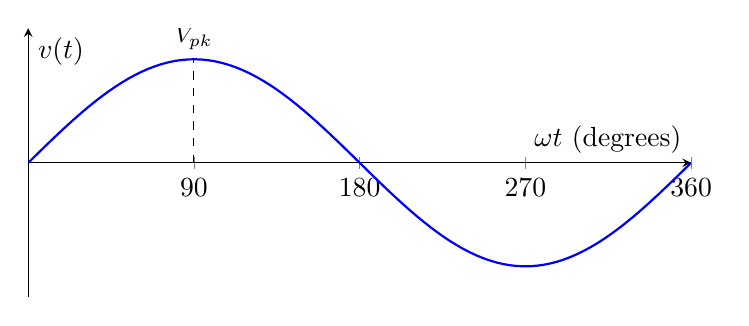
\begin{tikzpicture}[scale=1]
\begin{axis}[
  width=10cm, height=5cm,
  xlabel={$\omega t$ (degrees)}, ylabel={$v(t)$},
  xmin=0, xmax=360, ymin=-1.3, ymax=1.3,
  xtick={0,90,180,270,360}, ytick=\empty,
  axis lines=middle, samples=100,
  domain=0:360,
  enlargelimits=false
]
\addplot[thick,blue] {sin(x)};
\draw[dashed] (axis cs:90,0) -- (axis cs:90,1) node[above] {\footnotesize $V_{\text{pk}}$};
\end{axis}
\end{tikzpicture}
\end{center}

\subsection{Period and Frequency}

The \textbf{period} $T$ is the time for one complete cycle; frequency is
its reciprocal:
\[
\boxed{f = \frac{1}{T}} \qquad [\text{hertz, Hz} = \text{cycles per second}]
\]
A 14\,MHz signal completes $14\times10^{6}$ cycles every second, so its
period is $T = 1/(14\times10^{6}) \approx 71.4\,\text{ns}$.

\subsection{Amplitude Measures}

A sine wave can be described by several different amplitude measures,
and confusing them is one of the most common sources of error in AC
calculations:

\begin{center}
\begin{tabular}{@{}lll@{}}
\toprule
Measure & Meaning & Relation to $V_{\text{pk}}$ \\
\midrule
Peak ($V_{\text{pk}}$) & Maximum instantaneous value & --- \\
Peak-to-peak ($V_{\text{pp}}$) & Total swing, trough to crest & $V_{\text{pp}} = 2V_{\text{pk}}$ \\
RMS ($V_{\text{rms}}$) & Effective (heating) value & $V_{\text{rms}} = V_{\text{pk}}/\sqrt{2}$ \\
Average ($V_{\text{avg}}$) & Mean of the rectified waveform & $V_{\text{avg}} = 2V_{\text{pk}}/\pi$ \\
\bottomrule
\end{tabular}
\end{center}

\begin{keyidea}[Why RMS matters]
The \textbf{root-mean-square (RMS)} value of an AC waveform is defined so
that it produces the \emph{same heating effect} (the same average power
dissipation in a resistor) as a DC voltage of the same numerical value.
All of the DC power formulas from Chapter~\ref{ch:electricity}
($P=UI$, $P=I^2R$, $P=U^2/R$) apply directly to AC \emph{if} RMS values
are used for $U$ and $I$. Unless stated otherwise, voltages and currents
quoted for AC mains, transmitter output, and test equipment readings are
always RMS values.
\end{keyidea}

For a pure sine wave, $V_{\text{rms}} = V_{\text{pk}}/\sqrt{2} \approx
0.707\,V_{\text{pk}}$. This factor of $1/\sqrt2$ comes from averaging
$\sin^2(\theta)$ over a full cycle, which equals $\tfrac12$.

\begin{examplebox}[RMS conversion]
A sine wave has a peak voltage of 325\,V (typical of 230\,V AC mains).
Find its RMS value.

\emph{Solution.}
\[
V_{\text{rms}} = \frac{V_{\text{pk}}}{\sqrt2} = \frac{325}{1.414} \approx 230\,\text{V}.
\]
This confirms that ``230\,V mains'' is quoted as an RMS value.
\end{examplebox}

\section{Phase}

\textbf{Phase} describes the timing relationship between two waveforms of
the same frequency. Two sine waves are \textbf{in phase} if their peaks
and zero-crossings line up exactly ($\phi = 0$); they are \textbf{out of
phase} by however many degrees (or radians) one is shifted relative to
the other. A phase difference of $90\degree$ is described as
\textbf{quadrature}; $180\degree$ means the waveforms are exact mirror
images of each other (in \textbf{antiphase}).

Phase becomes critical once reactive components are introduced
(Chapters~\ref{ch:capacitors}--\ref{ch:rlc-resonance}): unlike a
resistor, a capacitor or inductor shifts the phase between the voltage
across it and the current through it, which is the origin of
\textbf{reactance} and \textbf{impedance}.

\section{The Rotating Phasor Picture}

A sine wave can be visualized as the vertical projection of a vector (a
\textbf{phasor}) of length $V_{\text{pk}}$ rotating counterclockwise at
angular velocity $\omega$. This picture --- formalized using complex
numbers as $V_{\text{pk}}e^{j(\omega t + \phi)}$ --- turns AC circuit
analysis into algebra: instead of tracking a continuously varying
instantaneous voltage, engineers track a fixed complex number (magnitude
and phase) per frequency, and the differential-equation relationships
between voltage and current across capacitors and inductors become
simple multiplication by a complex impedance. This is the ``$j$''
notation used throughout Chapters~\ref{ch:capacitors}--\ref{ch:rlc-resonance}.

\section{Why Sine Waves Are Special}

Sine waves are the natural output of resonant physical systems (a
pendulum, a vibrating string, an LC oscillator) and, crucially, are the
\emph{only} waveform shape that a linear circuit (one built from
resistors, capacitors, and inductors) cannot distort --- passing a sine
wave through a linear filter changes its amplitude and phase but never
its fundamental shape. This property, combined with the mathematical fact
that \emph{any} periodic waveform can be built from a sum of sine waves
at different frequencies (Fourier's theorem, Chapter~\ref{ch:non-sine}),
is why sinusoidal analysis is the foundation for understanding every
other waveform used in radio.

\begin{quickreview}
\item $v(t) = V_{\text{pk}}\sin(\omega t + \phi)$, with $\omega = 2\pi f$
and $f = 1/T$.
\item $V_{\text{pp}} = 2V_{\text{pk}}$; $V_{\text{rms}} =
V_{\text{pk}}/\sqrt2 \approx 0.707 V_{\text{pk}}$; DC power formulas apply
to AC when RMS values are used.
\item Phase describes timing offset between waveforms; $90\degree$ is
quadrature, $180\degree$ is antiphase.
\item The rotating phasor (complex-exponential) picture turns AC analysis
into algebra with complex numbers.
\item Any periodic waveform is a sum of sine waves at different
frequencies (previewing Fourier analysis, Chapter~\ref{ch:non-sine}).
\end{quickreview}

\begin{practiceproblems}
\item A sine wave has $V_{\text{rms}} = 120\,\text{V}$. Find
$V_{\text{pk}}$ and $V_{\text{pp}}$.
\item Find the period of a 7.100\,MHz signal.
\item Two sine waves of the same frequency have a phase difference of
$90\degree$. What term describes this relationship?
\item A signal generator is set to 1\,kHz with a peak amplitude of 5\,V.
Write the instantaneous voltage $v(t)$ as an equation, assuming zero
phase offset.
\item Explain why AC voltmeters are calibrated to read RMS rather than
peak values.
\end{practiceproblems}
